\documentclass[a4paper,11pt,german,notitlepage]{report}
\usepackage{xcolor}
\usepackage{tabularx}
\usepackage{dclecture}
\usepackage{qrcode}
\usepackage{awesomebox}
\usepackage{circuitikz}
\usepackage[style=german, german=swiss]{csquotes}
\def\farbe{darkgray} %Hier Farbe definieren
\addbibresource{refs.bib}

\ctikzset{
    logic ports=ieee,
    logic ports/scale=0.8,
    logic ports/fill=lightgray
}

\usetikzlibrary{arrows,shapes.gates.logic.US,shapes.gates.logic.IEC,calc,positioning}

\graphicspath{{img/}}

% Extract Exercises

%\usepackage[active, generate=trigonometry_exercises, extract-env={ex}]{extract}
%\begin{extract}
%\usepackage{xcolor}
%\def\farbe{teal}
%\usepackage{dcexercisesnogrid}
%\exercisetrue
%\end{extract}


%%% Fancy Header and Footer
\renewcommand{\headrule}{\vbox to 0pt{\hbox to\headwidth{\color{\farbe}\rule{\headwidth}{1pt}}\vss}}
\pagestyle{fancy} %eigener Seitenstil
\fancyhf{} %alle Kopf- und Fu§zeilenfelder bereinigen
\fancyhead[C]{Informatik - Gymnasium 1. Klasse - Algorithmen Projekt - Container Sortieren} %Kopfzeile mitte
%\fancyhead[R]{\includegraphics[width=0.2cm]{x.png}}

\fancyfoot[C]{\thepage}

%\rfoot{\setlength{\unitlength}{1mm}
%\begin{picture}(0,0)
%\put(5,0){\includegraphics{pic\thepage.ps}}
%\end{picture}}


\parskip=.1cm
\parindent=0cm
\linespread{1.5}



\begin{document}

\section*{Beschreibung}
In diesem Projekt nehmen Sie die Rolle einer Hafenverwaltungsfirma Colorbox ein.
Ihr Ziel ist es einen Kran zu programmieren, welcher die Container nach Farbe sortiert, damit die Container effizient auf Schiffe verladen werden können.
Jede Farbe entspricht hier einer Destination, zu welcher ein Container verfrachtet werden sollte.\\

\begin{figure}[h!]
    \centering
    
\includegraphics[height=3cm]{logo.png}  
\end{figure}

Als Notation für dieses Problem verwenden wir die Position der Stellplätze.
In der Vorlage haben Sie drei Stellplätze.
Wir teilen jedem Stellplatz von links aus eine Zahl beginnend bei $0$ zu.
Die Stellplätze sind also $0,1,2$.
Wenn Sie einen Container von Stellplatz $1$ zu Stellplatz $0$ bewegen, wäre die Notation dazu $(1,0)$ (von Platz 1 zu Platz 0).
Ein Container kann nicht von einem Stellplatz zum gleichen Stellplatz gelegt werden, da dann ja der gleiche Zustand erreicht würde.
Das bedeutet, das Beispielsweise der Zug $(0,0)$ nicht relevant ist.
Im gezeigten Beispiel gäbe es vier legale Züge: $(0,1),(0,2),(1,1),(1,2)$. Die Züge $(2,0)$ und $(2,1)$ wären nicht legal, da auf dem Stellplatz $2$ kein Container steht.

\begin{figure}[h!]
    \centering
    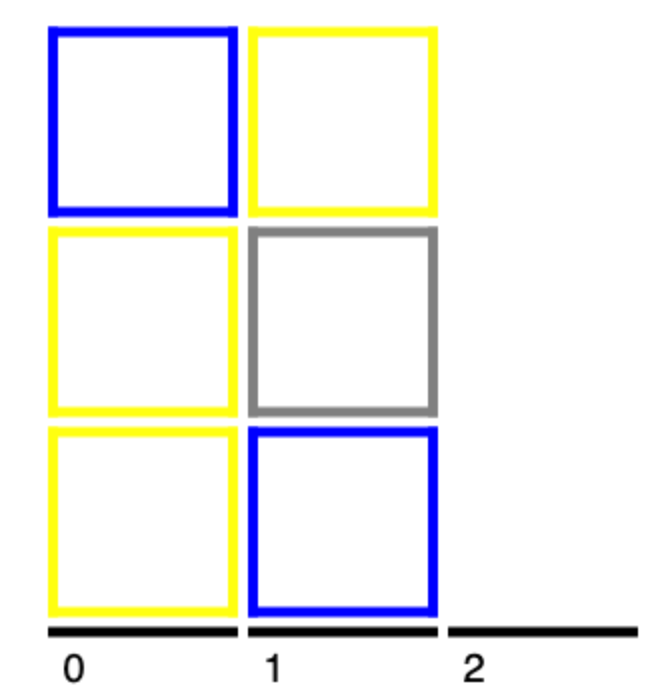
\includegraphics[width=5cm]{container.png}    
    \caption{Screenshot von WebTigerJython. Die Stellplätze sind unten (schwarz) und die Container stehen auf den Stellplätzen $0$ und $1$. Der Stellplatz $2$ ist hier leer.}
\end{figure}

Sie beginnen bereits mit einer implementierten Suche in der Codevorlage.
Diese Suche ist jedoch extrem ineffizient.
Nach 5000 durchsuchten Zuständen bricht das Program ab, um Ihren Computer zu schonen.
Es kann also sein, dass die Suche keine Lösung findet.
\section*{Regeln}
\begin{description}
    \item[Ziel:] Auf jedem Stellplatz sollen immer nur Container einer Farbe stehen, damit Sie effizient verladen werden können.
    \item[Züge:] Ihr Kran kann jeweils nur einen einzigen Container aufheben und an eine andere Position bewegen. 
\end{description}

\section*{Aufgabe}
Hier werden zusätzliche Aufgaben beschrieben, welche spezifisch für Ihr Projekt sind.
Die Aufgaben sind in zwei Gruppen unterzeilt: Pflichtaufgaben und optionale Aufgaben.
Die Pflichtaufgaben sollen am Ende des Projektes beantwortet sein.
Die optionalen Aufgaben dienen dazu, sich weiter im Thema zu vertiefen.
Diese Aufgaben sind Vorschläge. Sie dürfen auch eigene Fragestellungen vertiefen.
Deklarieren Sie Ihre Fragestellungen klar im Projektbericht.
Für alle Projekt gilt natürlich, dass Sie zuerst die allgemeine Aufgabenstellung und den Code (falls vorhanden) verstehen sollten, bevor Sie die untenstehen Aufgaben bearbeiten.
\subsection*{Pflichtaufgaben}
\begin{itemize}
    \item In der Vorlage ist bereits eine Suche Implementiert. Vergleichen Sie diese Suche mit dem manuellen Eingeben einer Lösung. Was fällt auf? Um was für einen Algorithmus könnte es sich handeln?
    \item Schreiben Sie ein Programm (oder verbessern Sie das existierende), welches jeweils eine optimale Lösung für Ihr Problem findet.
    \item (Falls Sie eine Breitensuche implementiert haben): Erweitern Sie das Problem, indem Sie in der Konfiguration mehr Container hinzufügen. Finden Sie mit der Breitensuche noch eine Lösung? Begründen Sie.
\end{itemize}
\subsection*{Optionale Aufgaben}
\begin{itemize}
    \item Implementieren Sie eine Heuristik, welcher jedem Zug angibt, wie gut er ist. Begründen Sie, warum Sie Ihre Heuristik gewählt haben.
    \item Implementieren Sie Ihre Heuristik als in einem Suchalgorithmus.
    \item Was passiert mit dem Problem, Wenn Ihr Kran nun mehr als einen Container von oben gleichzeitig aufheben kann?
    \item (Sehr schwierig!) Implementieren Sie eine Suche, welche das Aufheben mehrerer Container in betracht zieht.
\end{itemize}

\end{document}  
